%Este trabalho está licenciado sob a Licença Atribuição-CompartilhaIgual 4.0 Internacional Creative Commons. Para visualizar uma cópia desta licença, visite http://creativecommons.org/licenses/by-sa/4.0/deed.pt_BR ou mande uma carta para Creative Commons, PO Box 1866, Mountain View, CA 94042, USA.

\chapter{Vetores}\label{cap_vetor}

Neste capítulo, seguimos uma abordagem geométrica para introduzir os conceitos fundamentais e as operações básicas envolvendo vetores.

\section{Segmentos orientados}\label{cap_vetor_sec_segorien}

O conceito de \hl{\emph{segmento orientado}} é fundamental na definição de vetores. Como o próprio nome indica, \hl{trata-se de definir uma orientação a um dado \emph{segmento de reta}}. Antes, portanto, vamos definir o que entendemos por um segmento.

\subsection{Segmento}

\begin{flushright}
  [YouTube] | \href{https://archive.org/details/definicao-de-segmento}{[Vídeo]} | [Áudio] | \href{https://phkonzen.github.io/notas/contato.html}{[Contatar]}
\end{flushright}

\hl{Sejam dados dois pontos $A$ e $B$ sobre uma reta $r$. O conjunto de todos os pontos de $r$ entre $A$ e $B$ é chamado de \emph{segmento} e denotado por $AB$.} A reta $r$ é chamada de \emph{reta suporte} e os pontos $A$ e $B$ de \emph{pontos extremos}. Consulte a Figura~\ref{cap_vetor_sec_segorien:fig:segmento}.

\begin{figure}[H]
  \centering
  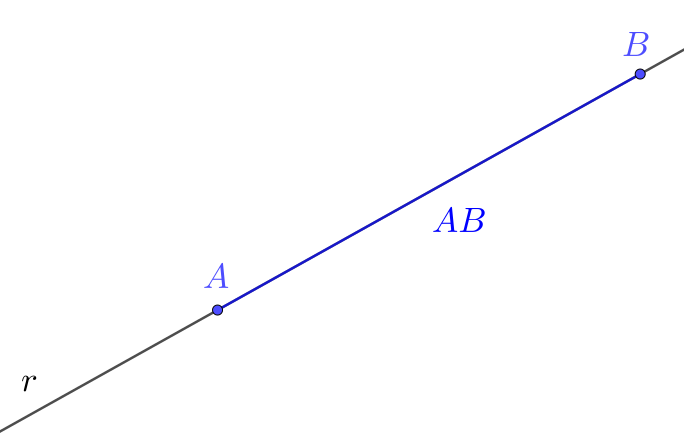
\includegraphics[max width=0.9\textwidth, max height=6in]{./cap_vetor/dados/fig_segmento/fig.png}
  \caption{Um segmento $AB$ de uma reta $r$.}
  \label{cap_vetor_sec_segorien:fig:segmento}
\end{figure}

\subsubsection{Norma e direção}

\hl{A \emph{norma} de um segmento $AB$ é denotada por $|AB|$ e definida como a distância entre seus pontos extremos $A$ e $B$}. Em outras palavras, é o tamanho ou comprimento do segmento\mynote{Em aplicações, a norma é medida em unidades de comprimento, metro $(m)$, no sistema internacional de unidades (SI).}.

\hl{A \emph{direção} de um segmento $AB$ é a direção de sua reta suporte, i.e. a direção da reta que fica determinada pelos pontos $A$ e $B$}. Logo, dois segmentos $AB$ e $CD$ têm a mesma direção, quando suas retas suportes são paralelas ou coincidentes (ou seja, elas têm a mesma direção).

\begin{ex}\label{cap_vetor_sec_segorien:ex:segmento}
  Consideramos os segmentos representados na Figura~\ref{cap_vetor_sec_segorien:fig:ex_segmento}. Observamos que $AB$ e $CD$ têm as mesmas direções, mas normas diferentes. Já, o segmento $EF$ tem a mesma norma que $AB$ (verifique!), mas tem direção diferente dos segmentos $AB$ e $CD$.
  
  \begin{figure}[H]
    \centering
    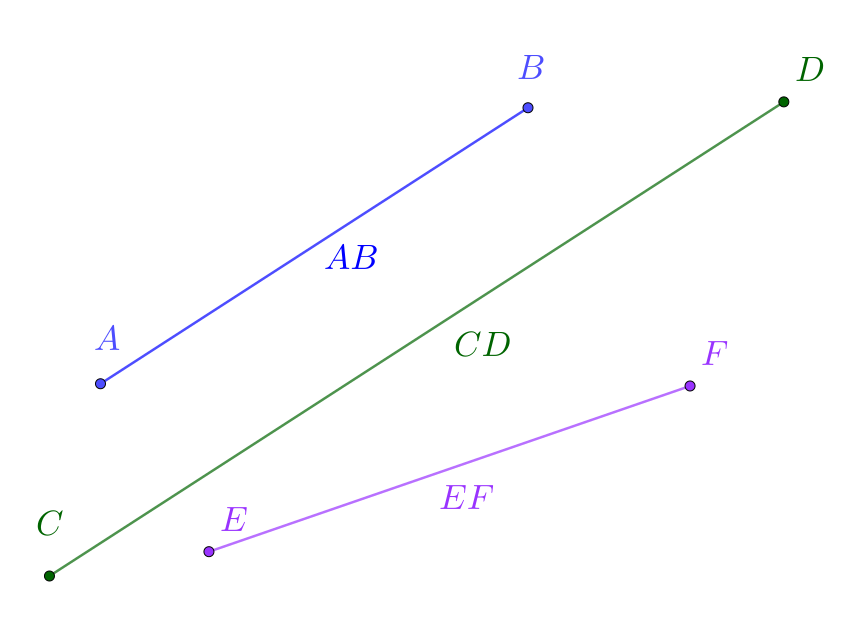
\includegraphics[max width=0.9\textwidth, max height=6in]{./cap_vetor/dados/fig_ex_segmento/fig.png}
  \caption{Segmentos de diferentes normas e direções.}
  \label{cap_vetor_sec_segorien:fig:ex_segmento}
\end{figure}
\end{ex}

% ESTOU AQUI!!!

\subsubsection{Segmento nulo}

Se $A$ e $B$ são pontos coincidentes, então chamamos $AB$ de \emph{segmento nulo} e temos $|AB| = 0$. Observamos que a representação geométrica de um segmento nulo é um ponto, tendo em vista que seus pontos extremos são coincidentes. Como existem infinitas retas de diferentes direções que passam por um único ponto, temos que segmentos nulos não têm direção definida.

\subsection{Segmento orientado}

\begin{flushright}
  \href{https://archive.org/details/definicao-segmento-orientado}{$\blacktriangleright$ Vídeo disponível!}
\end{flushright}

Observamos que um dado segmento $AB$ é igual ao segmento $BA$. Agora, podemos associar a noção de \emph{sentido} a um segmento, escolhendo um dos pontos como sua \emph{origem} (ou \emph{ponto de partida}) e o outro como sua \emph{extremidade} (ou \emph{ponto de chegada}). Ao fazermos isso, definimos um \emph{segmento orientado}.

Mais precisamente, um segmento orientado $AB$ é o segmento definido pelos pontos $A$ e $B$, sendo $A$ o ponto de partida (origem) e $B$ o ponto de chegada (extremidade). Veja a Figura \ref{fig:seg_orientado}.

\begin{figure}[H]
  \centering
  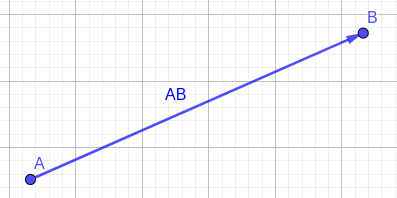
\includegraphics[width=0.5\textwidth]{./cap_vetor/dados/fig_seg_orientado/fig_seg_orientado}
  \caption{Esboço de um segmento orientado $AB$.}
  \label{fig:seg_orientado}
\end{figure}

\subsubsection{Norma e direção}

As noções de norma e de direção para segmentos estendem-se diretamente a segmentos orientados. Dizemos que dois dados segmentos orientados não nulos $AB$ e $CD$ têm a \textbf{mesma direção} quando as retas $AB$ e $CD$ são paralelas ou coincidentes. A norma de um segmento orientado $AB$ é a norma do segmento $AB$, denotada por $|AB|$. O segmento orientado nulo $AA$ tem norma $|AA|=0$ e não tem direção definida.

\begin{ex}\label{ex:segorien_direcao}
  Consideremos os segmentos orientados esboçados na Figura \ref{fig:ex_segorien_direcao}. Observemos que os segmentos orientados $AB$ e $CD$ têm a mesma direção. Já o segmento orientado $EF$ tem direção diferente dos segmentos $AB$ e $CD$.
  
  \begin{figure}[H]
    \centering
    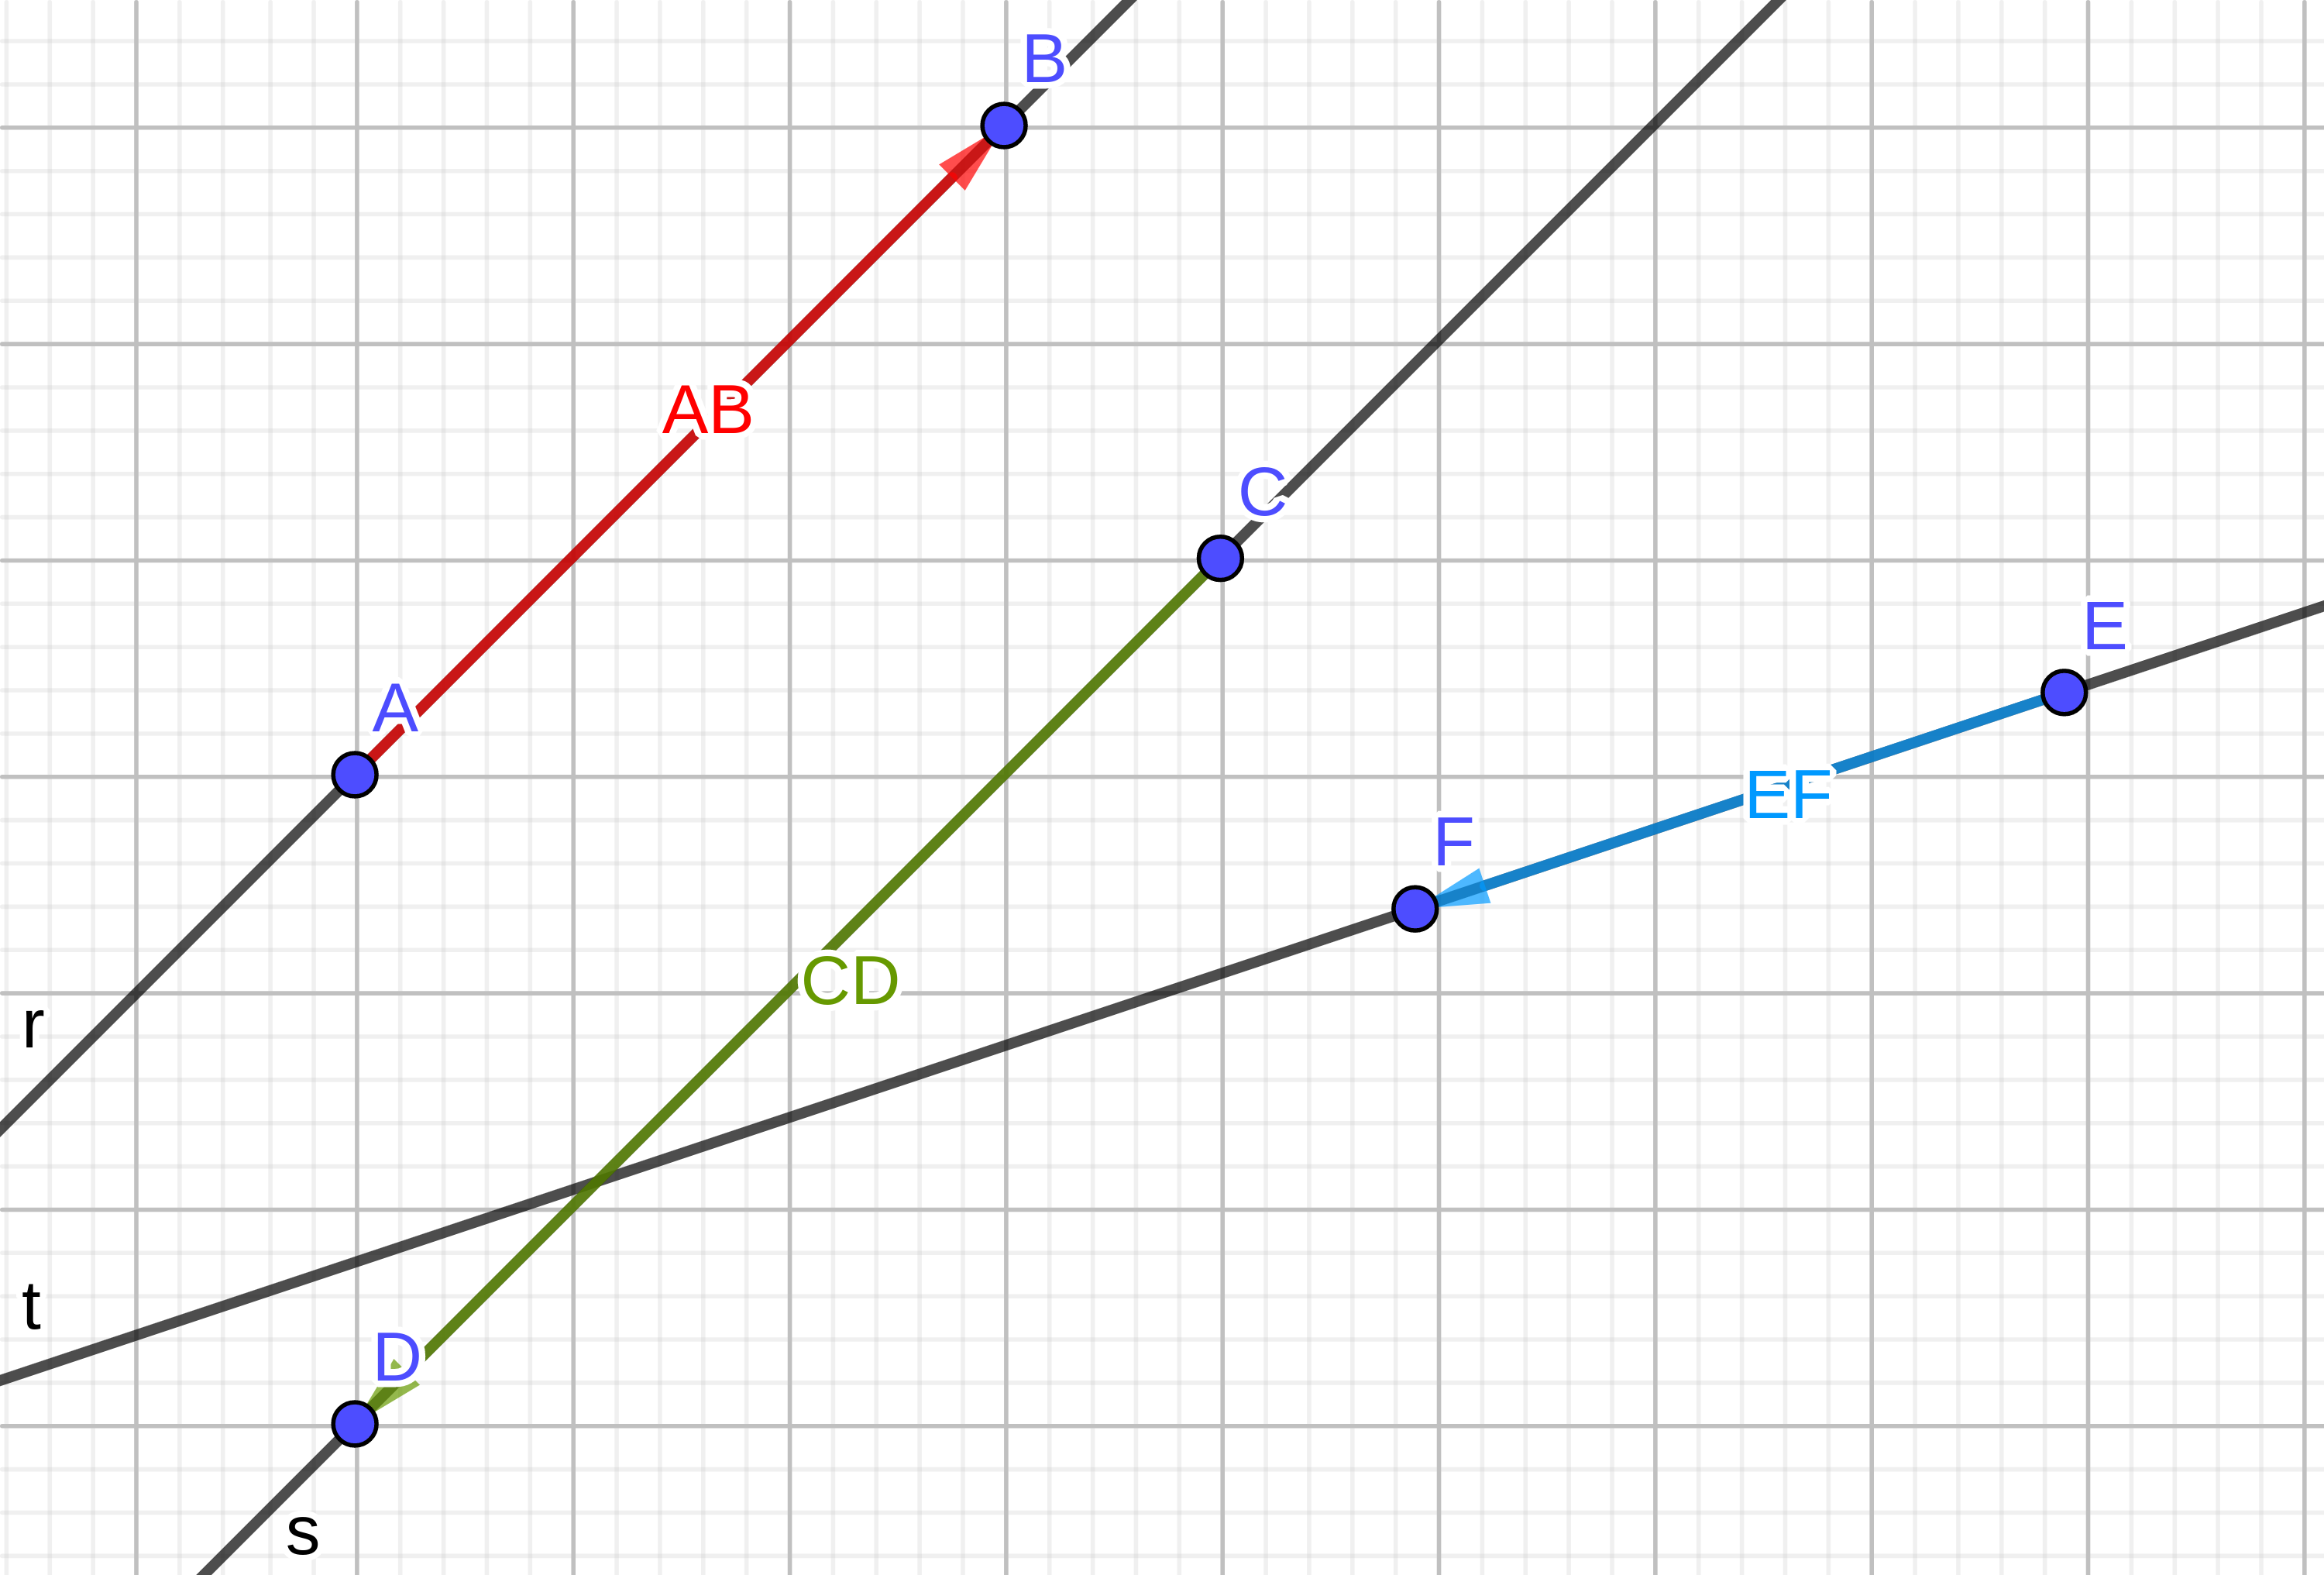
\includegraphics[width=0.7\textwidth]{./cap_vetor/dados/fig_ex_segorien_direcao/fig_ex_segorien_direcao}
  \caption{Esboço referente ao Exemplo \ref{ex:segorien_direcao}.}
  \label{fig:ex_segorien_direcao}
\end{figure}  
\end{ex}

\subsubsection{Comparação do sentido}

\begin{flushright}
  \href{https://archive.org/details/comparacao-sentido-segmentos-orientados}{$\blacktriangleright$ Vídeo disponível!}
\end{flushright}

Segmentos orientados $AB$ e $CD$ de mesma direção podem ter o mesmo sentido ou sentidos opostos. No caso de suas retas suportes não serem coincidentes, os segmentos orientados $AB$ e $CD$ têm a mesma direção, quando os segmentos $AC$ e $BD$ não se interceptam. E, caso estas se interceptam, os segmentos orientados $AB$ e $CD$ têm sentidos opostos. 

\begin{ex}
  Na Figura \ref{fig:segorien_sentido}, temos que os segmentos $AB$ e $CD$ têm o mesmo sentido. De fato, observamos que eles têm a mesma direção e que os segmentos $AC$ e $BD$ têm interseção vazia.

\begin{figure}[H]
  \centering
  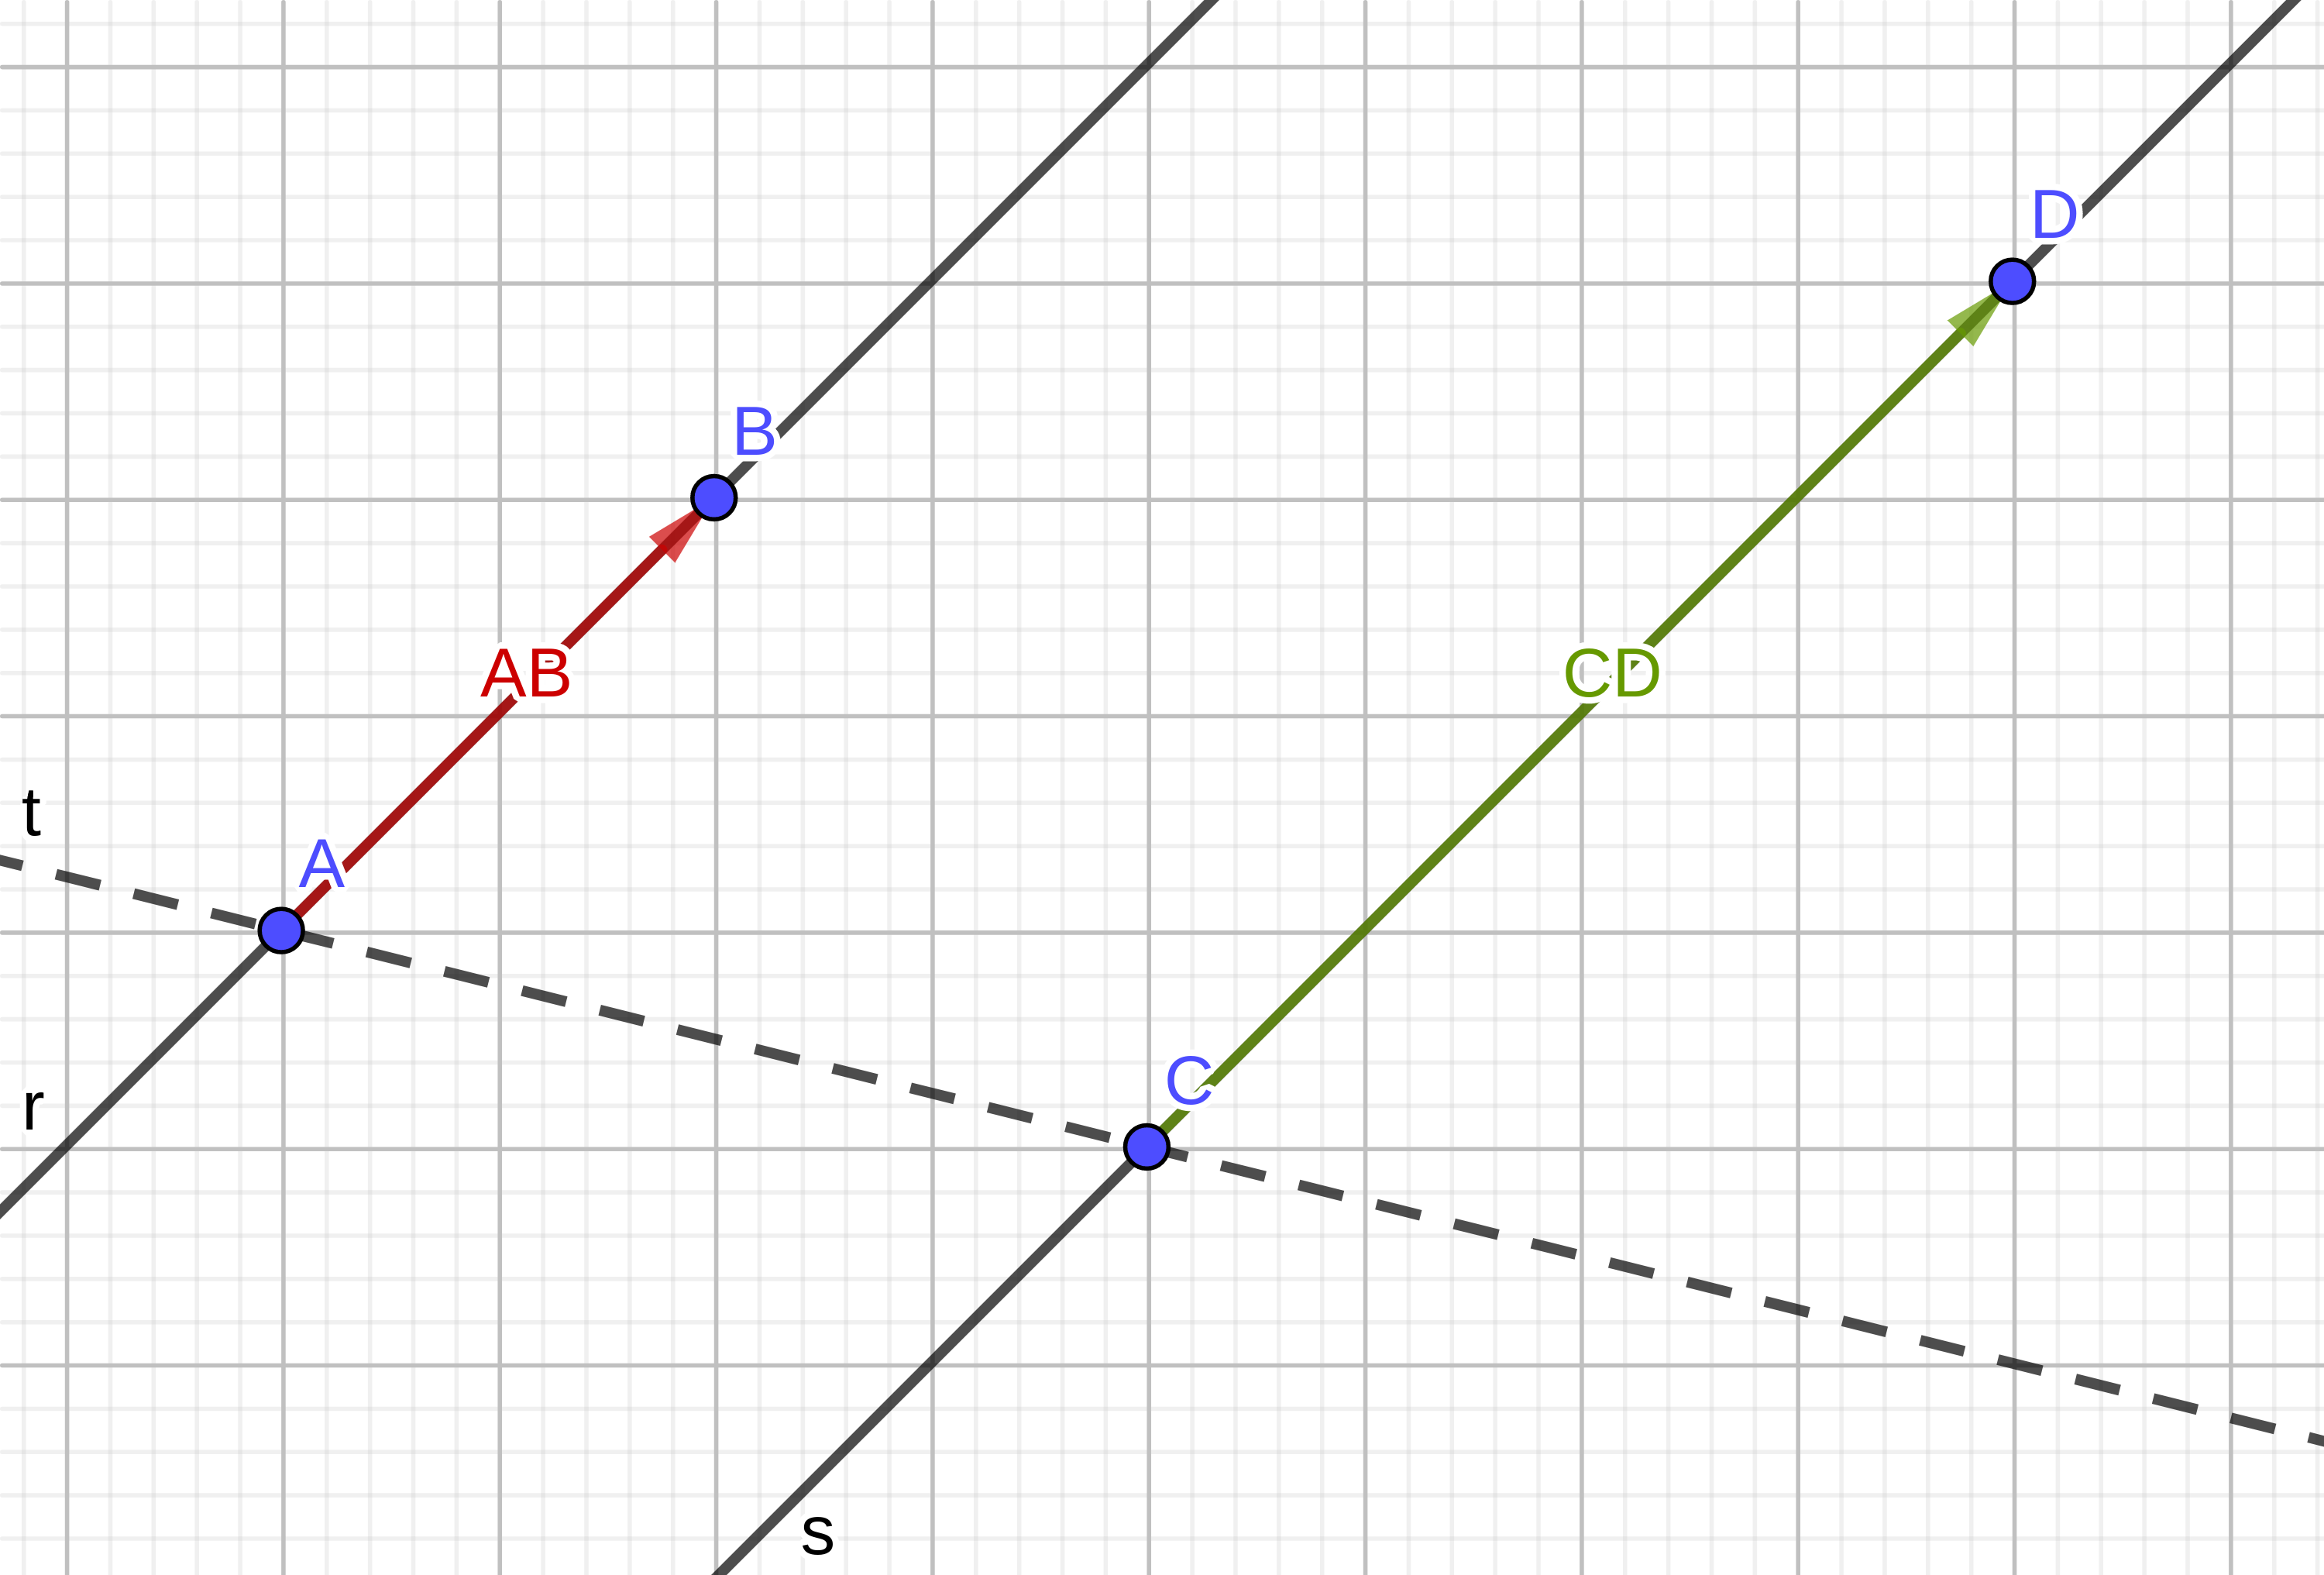
\includegraphics[width=0.7\textwidth]{./cap_vetor/dados/fig_segorien_sentido/fig_segorien_sentido}
  \caption{Segmentos orientados $AB$ e $CD$ de mesmo sentido. Segmentos orientados $EF$ e $GH$ de sentidos opostos.}
  \label{fig:segorien_sentido}
\end{figure}

Na mesma Figura \ref{fig:segorien_sentido}, vemos que os segmentos orientados $EF$ e $GH$ têm sentidos opostos, pois têm a mesma direção e os segmentos $EG$ e $FH$ se interceptam (no ponto $I$). 
\end{ex}

\begin{obs}\label{obs:segorin_sentido_trans}
  A propriedade de segmentos orientados terem o mesmo sentido é transitiva. Ou seja, se $AB$ e $CD$ têm o mesmo sentido e $CD$ e $EF$ têm o mesmo sentido, então $AB$ e $EF$ têm o mesmo sentido.
\end{obs}

Com base na Observação \ref{obs:segorin_sentido_trans}, analisamos o sentido de dois segmentos orientados e colineares escolhendo um deles e construindo um segmento orientado de mesmo sentido  e não colinear. Então, analisamos o sentido dos segmentos orientados originais com respeito ao introduzido.

\subsubsection{Equipolência}

\begin{flushright}
  \href{https://archive.org/details/segmentos-orientados-equipolentes}{$\blacktriangleright$ Vídeo disponível!}
\end{flushright}

Um segmento orientado não nulo $AB$ é \emph{equipolente} a um segmento orientado $CD$, quando $AB$ tem a \emph{mesma norma}, a \emph{mesma direção} e o \emph{mesmo sentido} de $CD$. Segmentos nulos também são considerados equipolentes entre si. Quando $AB$ é equipolente a $CD$, escrevemos $AB \sim CD$.

\begin{figure}[H]
  \centering
  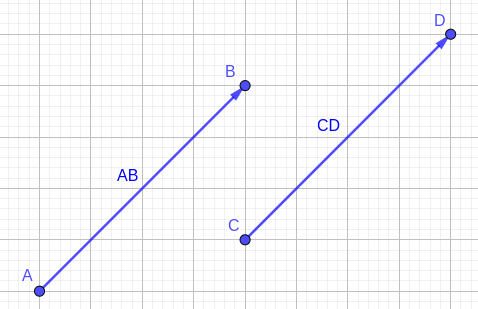
\includegraphics[width=0.7\textwidth]{./cap_vetor/dados/fig_segequipolentes/fig_segequipolentes}
  \caption{Esboço de dois segmentos orientados $AB$ e $CD$ equipolentes.}
  \label{fig:segequipolentes}
\end{figure}

A relação de equipolência é uma \emph{relação de equivalência}. De fato, temos:
\begin{itemize}
\item \emph{relação reflexiva}: $AB \sim AB$;
\item \emph{relação simétrica}: $AB \sim CD \Rightarrow CD \sim AB$;
\item \emph{relação transitiva}: $AB \sim CD ~ \text{e} ~ CD \sim EF \Rightarrow AB \sim EF$.
\end{itemize}

Com isso, dado um segmento $AB$, definimos a \emph{classe de equipolência} de $AB$ como o conjunto de todos os segmentos equipolentes a $AB$. O segmento $AB$ é um \emph{representante} desta classe.

\subsection{Exercícios resolvidos}

\begin{exeresol}
  Mostre que dois segmentos orientados $AB$ e $CD$ são equipolentes se, e somente se, os pontos médios de $AD$ e $BC$ são coincidentes.
\end{exeresol}
\begin{resol}
  Começamos mostrando a implicação. Por hipótese, temos que $AB$ e $CD$ são equipolentes. A tese é clara no caso de $AB$ e $CD$ serem coincidentes. Vejamos, então, o caso em que $AB$ e $CD$ não são coincidentes. Desta forma, $ABCD$ determina um paralelogramo de diagonais $AD$ e $BC$. Como as diagonais de um paralelogramo se interceptam em seus pontos médios, temos demonstrado a implicação.

  Agora, mostramos a recíproca. Por hipótese, temos que os pontos médios de $AD$ e $BC$ são coincidentes. Novamente, se $AD$ e $BD$ são coincidentes a conclusão é direta. Consideremos o caso em que $AD$ e $BD$ não são coincidentes. Daí, segue que $AB$ e $CD$ têm o mesmo tamanho e mesma direção. Seja $M$ o ponto médio de $AD$ e $BC$ e $\pi$ o plano determinado pelos segmentos $AB$ e $CD$. Notando que $M$, $B$ e $D$ estão no mesmo semiplano de $\pi$ determinado pela reta $AC$, concluímos que $AB$ e $CD$ são equipolentes.
\end{resol}

\begin{exeresol}
  Mostre que $AB\sim CD$, então $BA\sim DC$.
\end{exeresol}
\begin{resol}
  $AB$ e $BA$ têm o mesmo tamanho e direção. $CD$ e $DC$ têm o mesmo tamanho e direção. Como $AB\sim CD$, temos que $BA$ e $DC$ têm o mesmo tamanho e direção. Por fim, observa-se que $BA$ e $DC$ têm ambos o mesmo sentido oposto de $AB$ e $DC$. 
\end{resol}

\subsection{Exercícios}

\begin{exer}
  Faça o esboço de dois segmentos $AB$ e $CD$ com $|AB|\neq |CD|$ e cujas retas determinadas por eles sejam coincidentes.
\end{exer}

\begin{exer}
  Faça o esboço de dois segmentos orientados $AB\not\sim CD$ e de mesmo sentido.
\end{exer}

\begin{exer}
  Faça o esboço de dois segmentos orientados colineares, de tamanhos iguais e sentidos opostos.
\end{exer}

\begin{exer}
  Diga se é verdadeira ou falsa a seguinte afirmação: é quadrado todo trapézio retângulo $ABCD$ com segmentos orientados $AD$ e $BC$ equipolentes. Justifique sua afirmação. 
\end{exer}
\begin{resp}
  Falsa.
\end{resp}

\begin{exer}
  Mostre que $AB\sim CD$, então $AC\sim BD$.
\end{exer}
\begin{resp}
  Dica: $ABCD$ determina um paralelogramo.
\end{resp}

\begin{exer}
  Mostre que se $AC\sim CB$, então $C$ é ponto médio do segmento $AB$.
\end{exer}

\ifisbook
\subsubsection{Respostas}
\shipoutAnswer
\fi

\section{Vetor}\label{cap_vetor_sec_vetor}

\begin{flushright}
  \href{https://archive.org/details/definicao-vetor}{$\blacktriangleright$ Vídeo disponível!}
\end{flushright}

Dado um segmento orientado $AB$, define-se o vetor $\overrightarrow{AB}$ (lê-se vetor $AB$), a classe de equipolência de $AB$. Um segmento orientado da classe é um representante (geométrica) do vetor. A Figura \ref{fig:vetor} mostra duas representações de um dado vetor $\vec{u} = \overrightarrow{AB}$.

\begin{figure}[H]
  \centering
  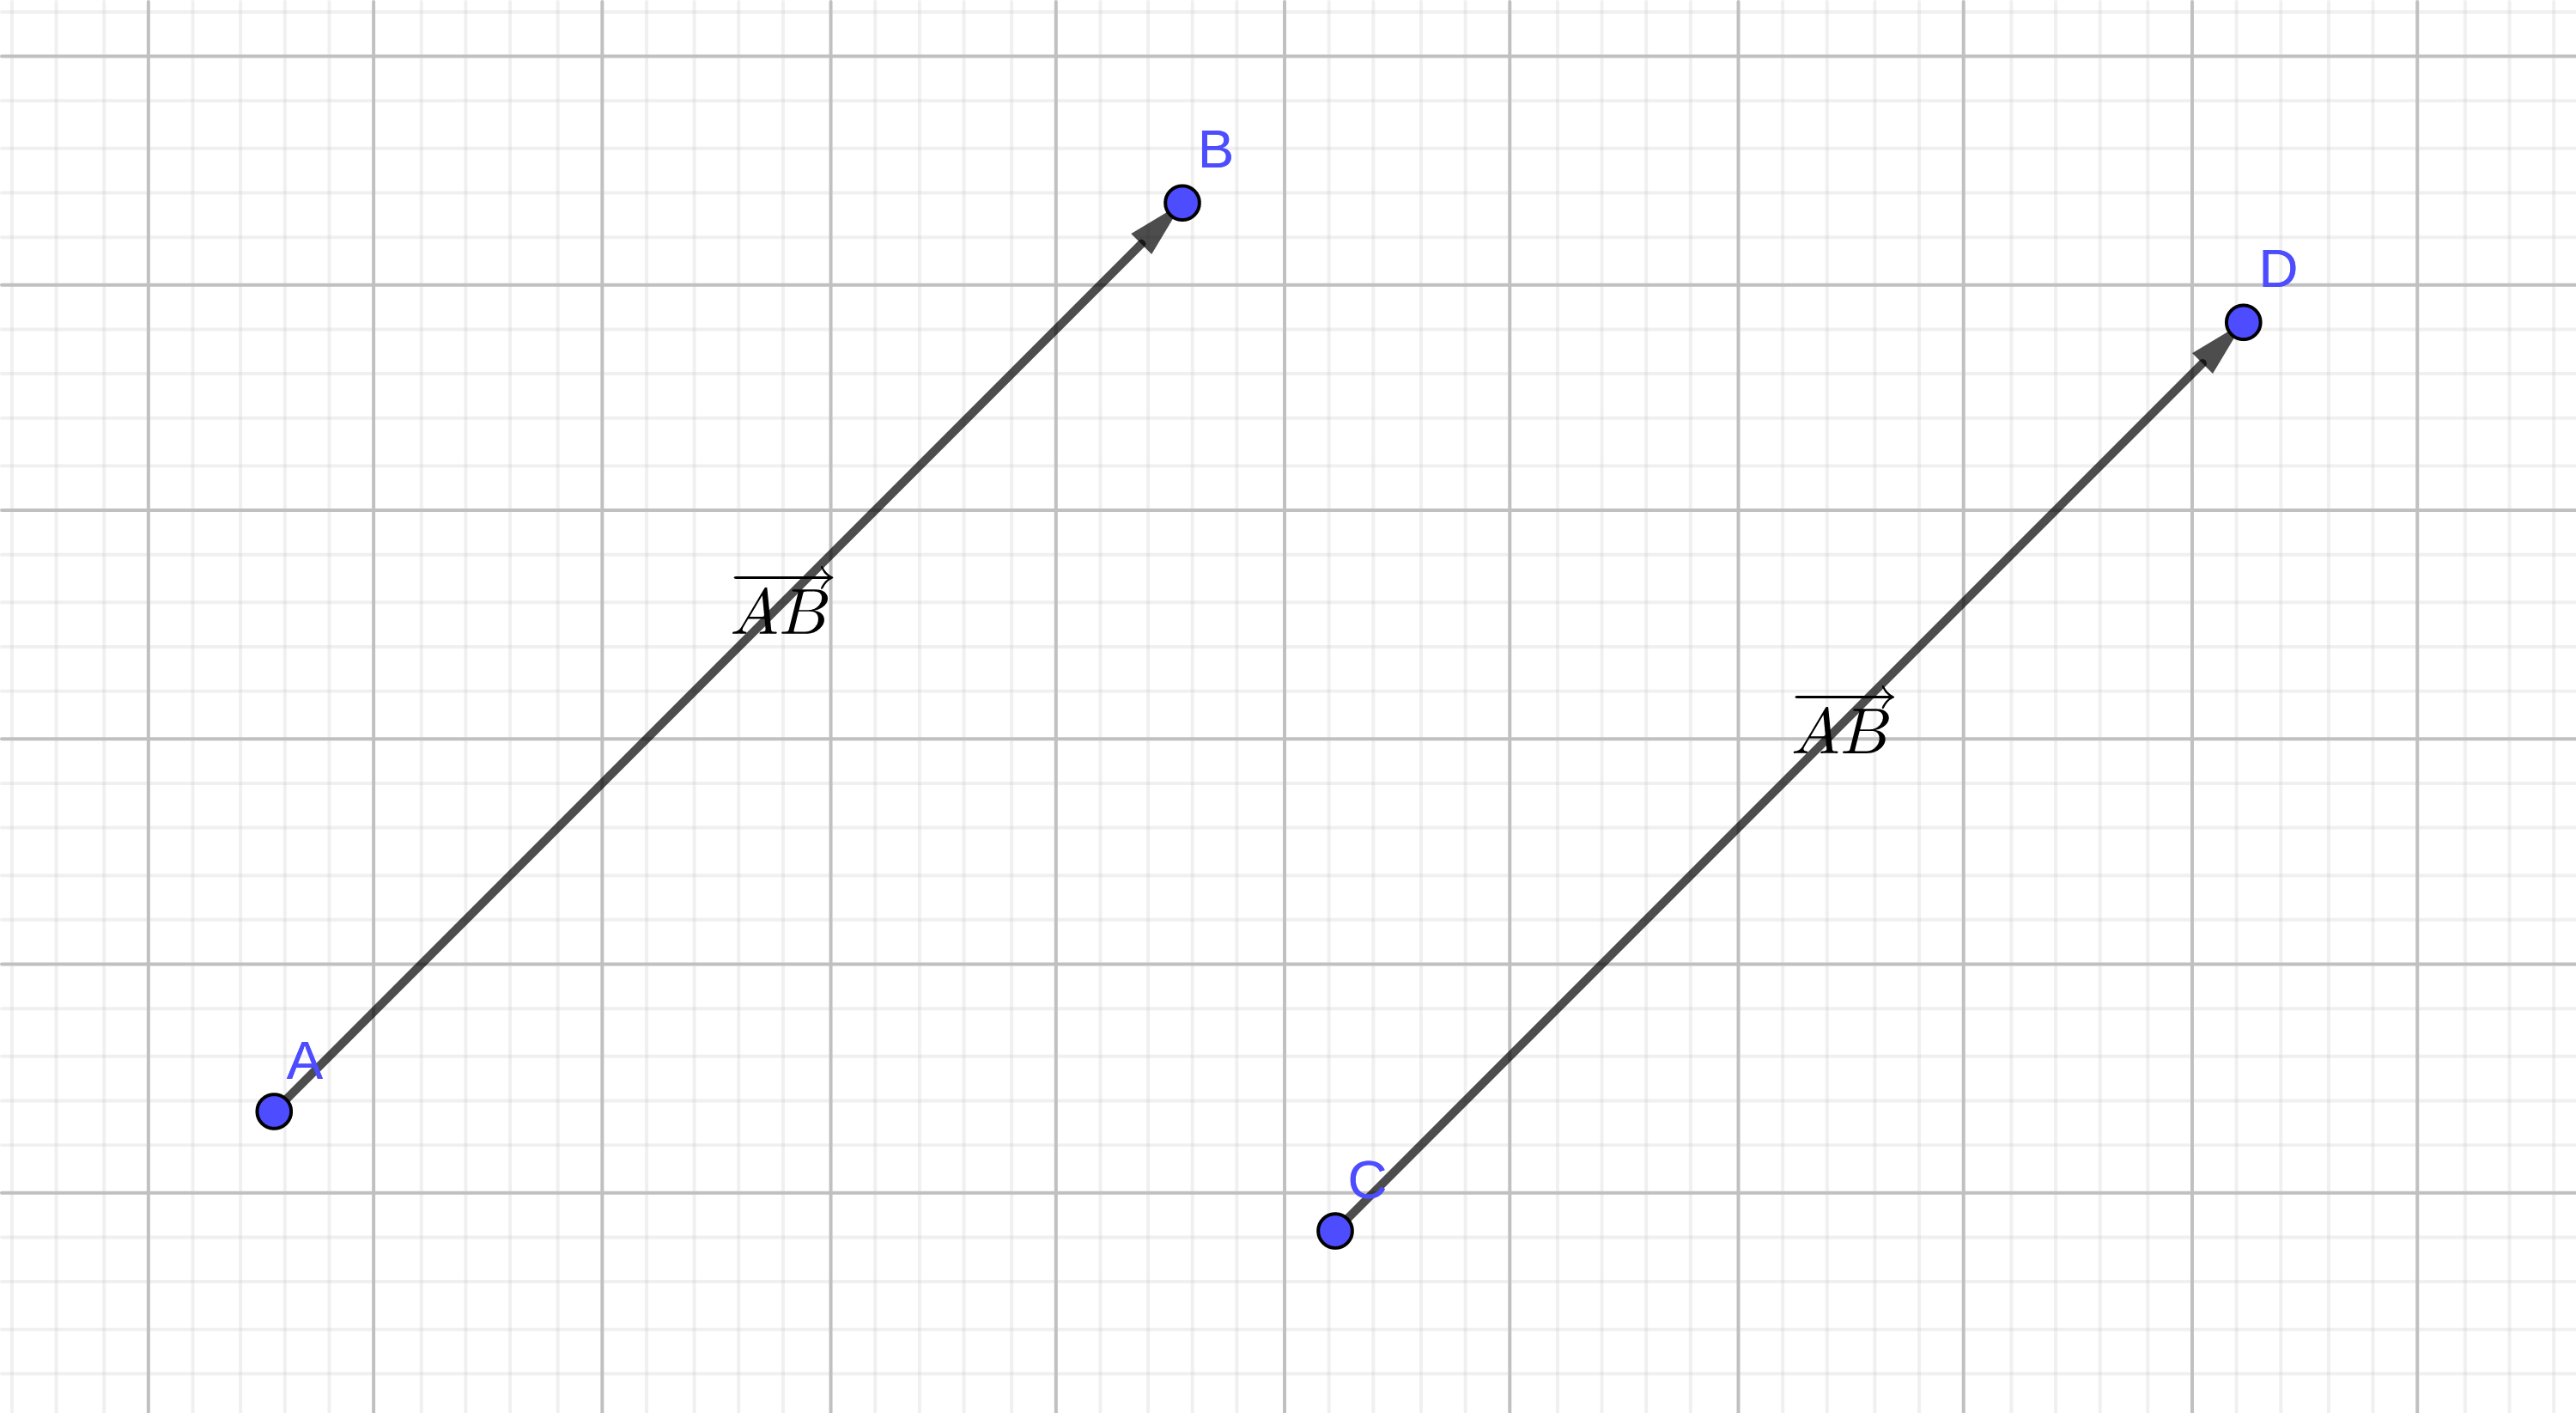
\includegraphics[width=0.7\textwidth]{./cap_vetor/dados/fig_vetor/fig_vetor}
  \caption{Esboço de duas representações de dado vetor $\vec{u}$.}
  \label{fig:vetor}
\end{figure}

O \emph{vetor nulo} é aquele que tem como representante um segmento orientado nulo. É denotado por $\vec{0}$ e geometricamente representado por um ponto.

A \emph{norma} (ou módulo) de um vetor $\vec{u}$ é denotada(o) por $|\vec{u}|$ e é definido como a norma de qualquer uma de suas representações. Mais precisamente, se o segmento orientado $AB$ é uma representação de $\vec{v}$, i.e. $\vec{v} = \overrightarrow{AB}$, então
\begin{equation}
|\vec{v}| = |\overrightarrow{AB}| := |AB|
\end{equation}

\begin{obs}
  $|\vec{v}| = 0$ se, e somente se, $\vec{v} = \vec{0}$.

  Seja $\vec{v} = \overrightarrow{AB}$. Lembrando que $|\overrightarrow{AB}| = |AB|$, i.e. a distância entre os pontos $A$ e $B$, segue que se $\vec{v} = \vec{0}$, então $AB$ é um segmento orientado nulo e, portanto, $0=|AB|=|\vec{v}|$. Reciprocamente, se $|\vec{v}| = 0$, então $|AB| = 0$ e, portanto, $AB$ é um segmento orientado nulo, i.e. $A$ e $B$ são pontos sobrepostos (coincidentes) e $\overrightarrow{AB} = \vec{0}$.
\end{obs}

Dois \textbf{vetores} são ditos \textbf{paralelos} quando qualquer de suas representações têm a mesma direção. De forma análoga, definem-se \textbf{vetores coplanares}, \textbf{vetores não coplanares}, \textbf{vetores ortogonais}, além de conceitos como \textbf{ângulo entre dois vetores}, etc.


\begin{ex}
  Vejamos a Figura \ref{fig:vetorrel}. Temos os vetores paralelos $\vec{u}$ e $\vec{v}$, enquanto que os vetores $\vec{s}$ e $\vec{t}$ são ortogonais (ou perpendiculares).

  \begin{figure}[H]
    \centering
    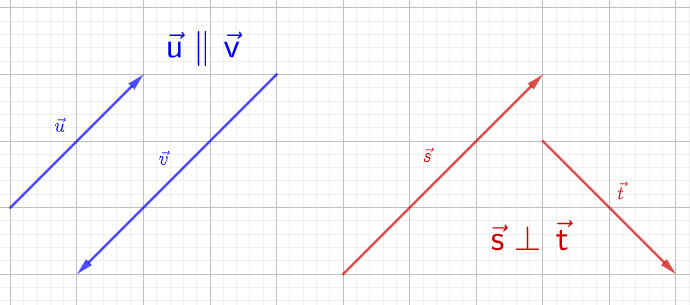
\includegraphics[width=0.7\textwidth]{./cap_vetor/dados/fig_vetorrel/fig_vetorrel.png}\\
    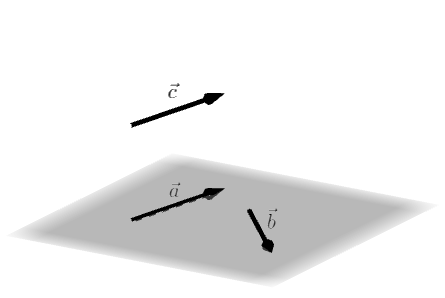
\includegraphics[width=0.5\textwidth]{./cap_vetor/dados/fig_vcolineares/fig_vcolineares.png}
    \caption{Esquerda: esboços de vetores paralelos e de vetores ortogonais. Direita: esboços de vetores coplanares.}
    \label{fig:vetorrel}
  \end{figure}
  
  Também da Figura \ref{fig:vetorrel}, temos que os vetores $\vec{a}$, $\vec{b}$ e $\vec{c}$ são coplanares. Embora, na figura $\vec{c}$ está representado fora do plano determinado pelas representações de $\vec{a}$ e $\vec{b}$, podemos tomar uma outra representação de $\vec{c}$ coplanar a estas representações.
\end{ex}


\subsection{Adição de vetores}

\begin{flushright}
  \href{https://archive.org/details/adicao-de-vetores}{$\blacktriangleright$ Vídeo disponível!}
\end{flushright}

Sejam dados dois vetores $\vec{u}$ e $\vec{v}$. Sejam, ainda, uma representação $\overrightarrow{AB}$ de $\vec{u}$ e uma representação $\overrightarrow{BC}$ do vetor $\vec{v}$. Então, define-se o vetor soma $\vec{u}+\vec{v}$ como o vetor representado por $\overrightarrow{AC}$. Veja a Figura \ref{fig:vadicao}.

\begin{figure}[H]
  \centering
  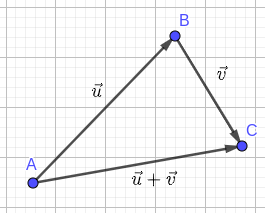
\includegraphics[width=0.5\textwidth]{./cap_vetor/dados/fig_vadicao/fig_vadicao}
  \caption{Representação geométrica da adição de dois vetores.}
  \label{fig:vadicao}
\end{figure}

\begin{obs}
  Vejamos as seguintes propriedades:
  \begin{enumerate}[a)]
  \item Elemento neutro na adição:
    \begin{equation}
      \vec{u} + \vec{0} = \vec{u}
    \end{equation}
    
    De fato, seja $\vec{u} = \overrightarrow{AB}$. Observamos que podemos representar $\vec{0} = \overrightarrow{BB}$. Logo, temos $\vec{u} + \vec{0} = \overrightarrow{AB} + \overrightarrow{BB} = \overrightarrow{AB} = \vec{u}$.

  \item Associatividade na adição:
    \begin{equation}
      (\vec{u} + \vec{v}) + \vec{w} = \vec{u} + (\vec{v} + \vec{w}).
    \end{equation}

    De fato, sejam $\vec{u} = \overrightarrow{AB}$, $\vec{v} = \overrightarrow{BC}$ e $\vec{w} = \overrightarrow{CD}$. Então, segue
    \begin{align}
      \left(\vec{u} + \vec{v}\right)+\vec{w} &= \left(\overrightarrow{AB}+\overrightarrow{BC}\right)+\overrightarrow{CD} \\
                                             &= \overrightarrow{AC} + \overrightarrow{CD} \\
                                             &= \overrightarrow{AD},
    \end{align}
    bem como,
    \begin{align}
      \vec{u} + \left(\vec{v} + \vec{w}\right) &= \overrightarrow{AB}+\left(\overrightarrow{BC}+\overrightarrow{CD}\right) \\
                                             &= \overrightarrow{AB} + \overrightarrow{BD} \\
                                             &= \overrightarrow{AD}.
    \end{align}
  \item Comutatividade da adição:
    \begin{equation}
      \vec{u} + \vec{v} = \vec{v} + \vec{u}.
    \end{equation}

    Esta propriedade pode ser demonstrada usando a regra do paralelogramo que veremos mais adiante. Veja, também, o Exercício Resolvido \ref{exeresol:vetor_comuta_adicao}.
  \end{enumerate}
\end{obs}

\subsection{Vetor oposto}

\begin{flushright}
  \href{https://archive.org/details/vetor-oposto}{$\blacktriangleright$ Vídeo disponível!}
\end{flushright}

Um \textbf{vetor} $\vec{v}$ é dito ser \textbf{oposto} a um dado vetor $\vec{u}$, quando quaisquer representações de $\vec{u}$ e $\vec{v}$ são segmentos orientados de mesmo comprimento e mesma direção, mas com sentidos opostos. Neste caso, denota-se por $-\vec{u}$ o vetor oposto a $\vec{u}$. Veja a Figura \ref{fig:voposto}.

\begin{figure}[H]
  \centering
  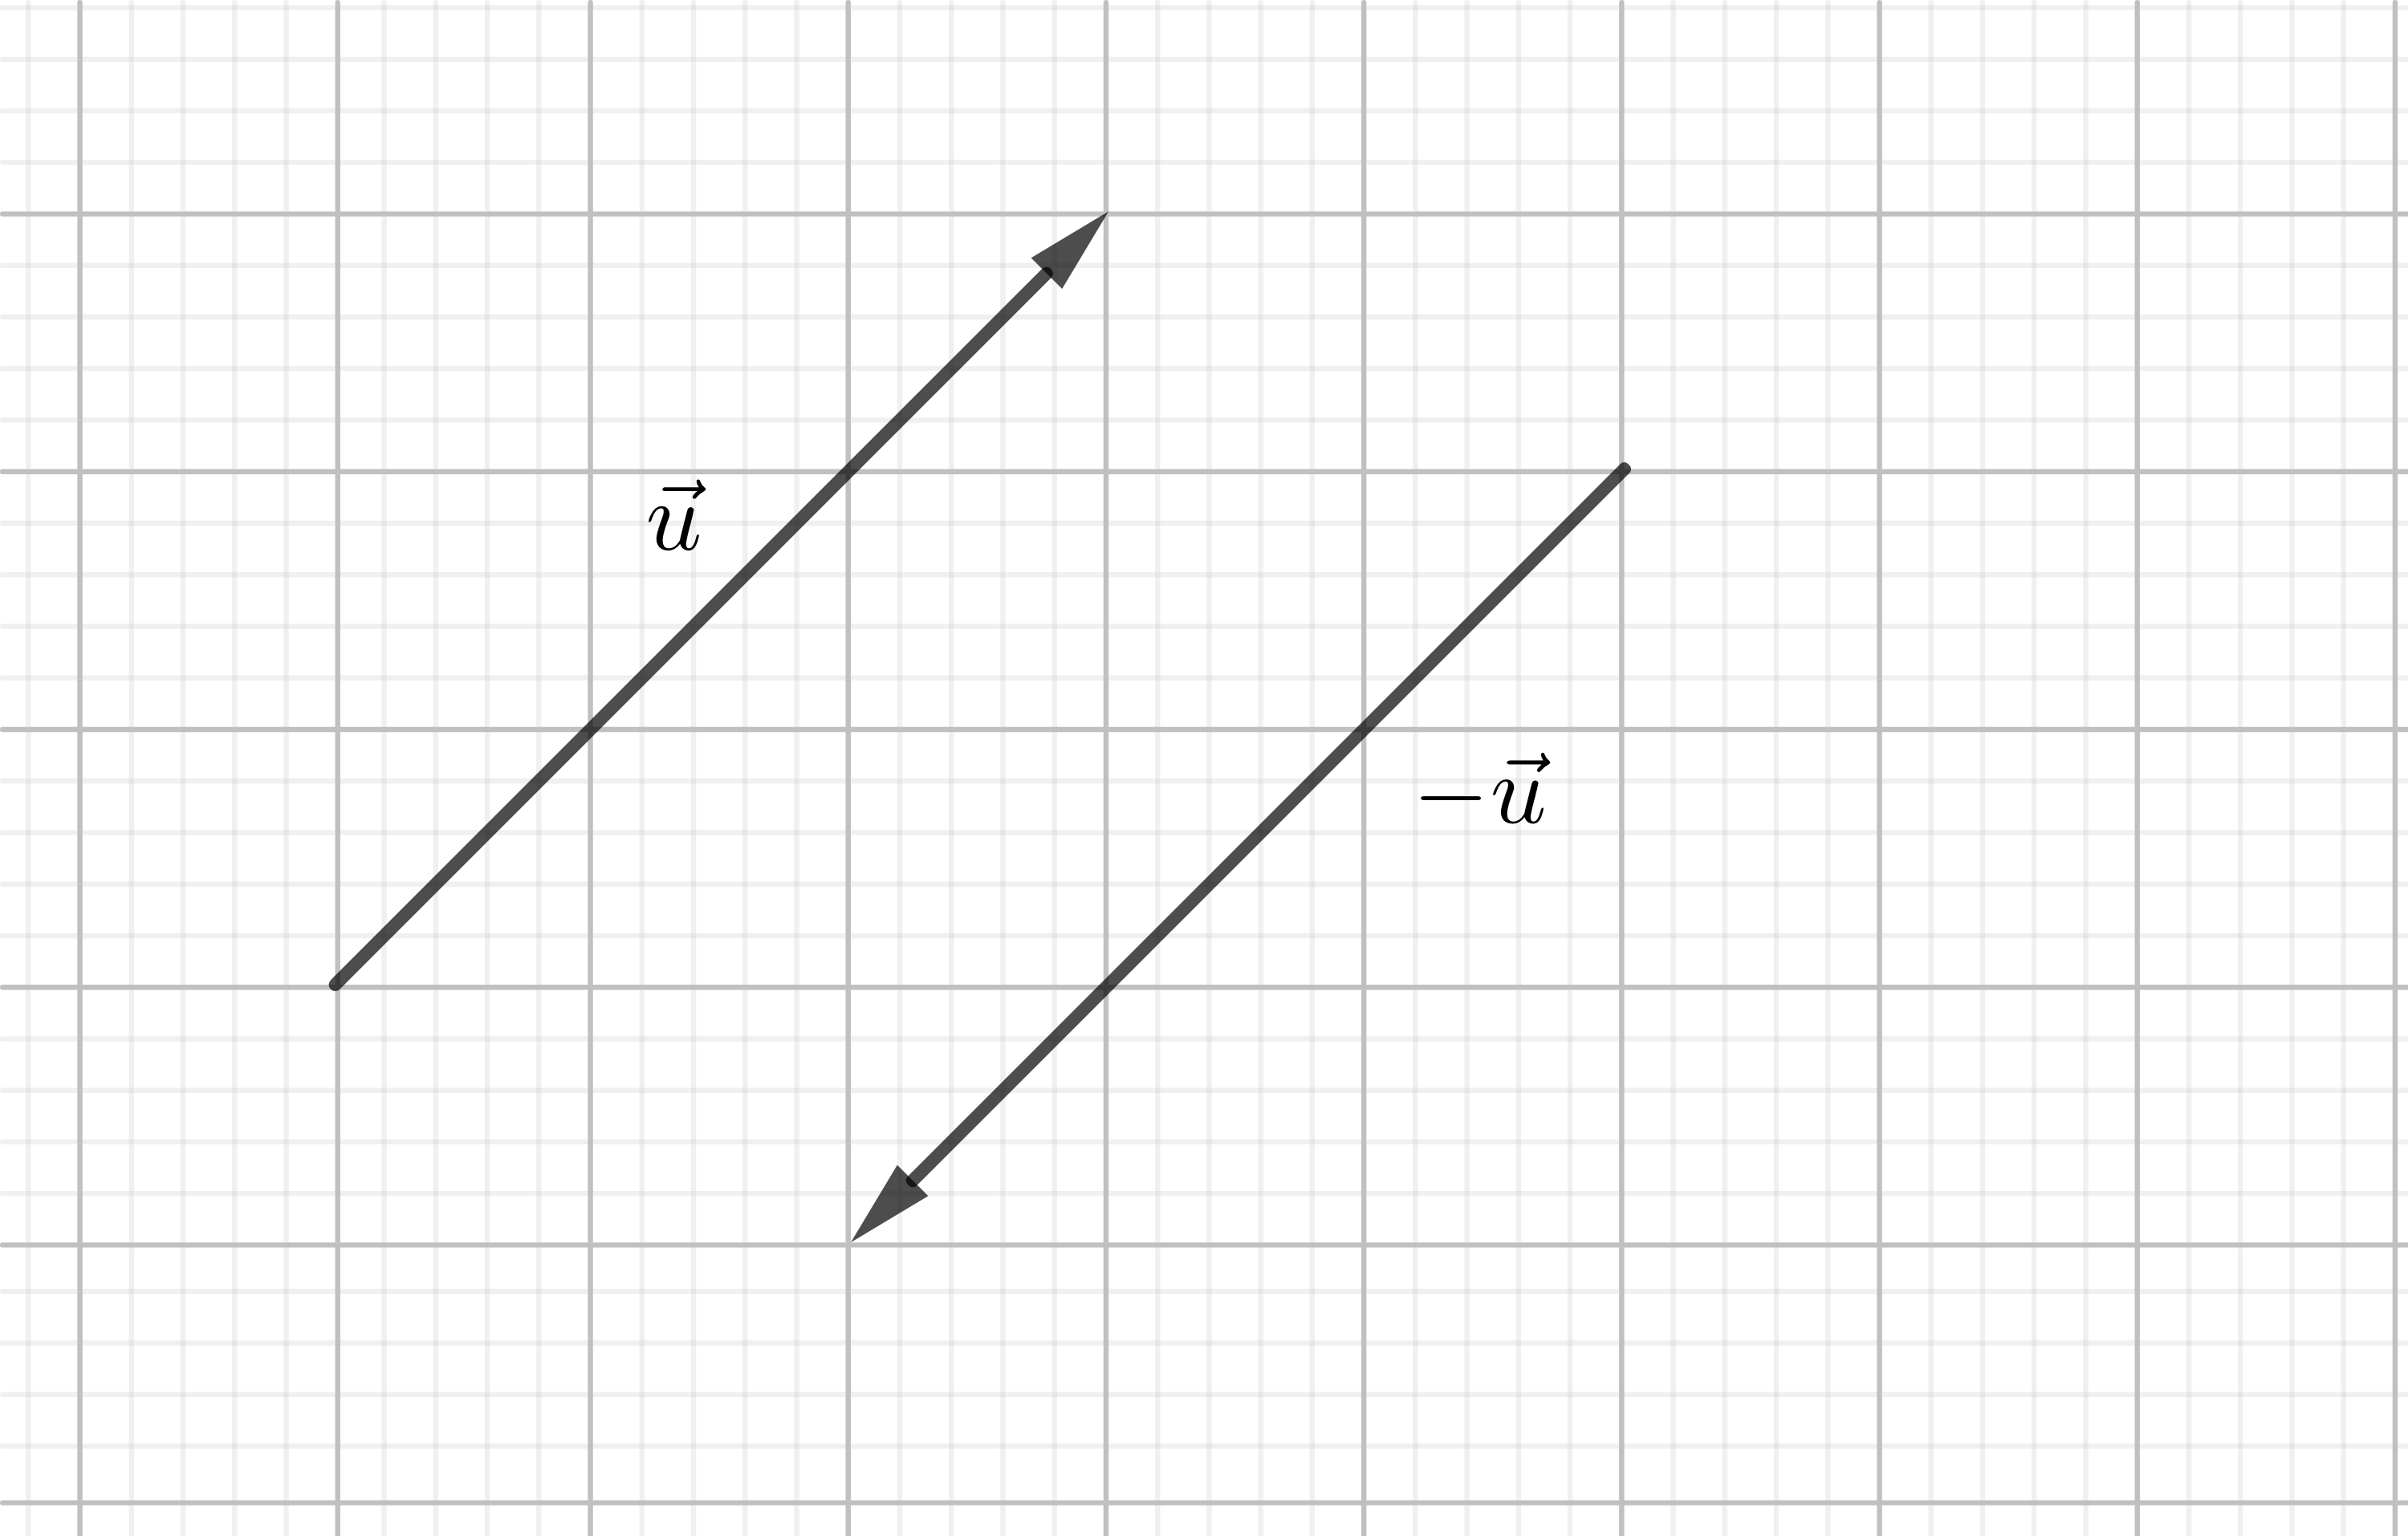
\includegraphics[width=0.5\textwidth]{./cap_vetor/dados/fig_voposto/fig_voposto}
  \caption{Representação geométrica de vetores opostos.}
  \label{fig:voposto}
\end{figure}

\begin{obs}
  $|\vec{v}| = |-\vec{v}|$.

  De fato, seja $\vec{v} = \overrightarrow{AB}$. Então, $|\vec{v}| = |AB| = |BA| = |-\vec{v}|$.
\end{obs}

\begin{obs}(Existência do oposto)
  \begin{equation}
    \vec{u} + \left(-\vec{u}\right) = \vec{0}.
  \end{equation}

  De fato, seja $\vec{u} = \overrightarrow{AB}$. Então, $-\vec{u} = -\overrightarrow{AB} = \overrightarrow{BA}$. Segue que
  \begin{align}
    \vec{u} + \left(-\vec{u}\right) &= \overrightarrow{AB} + \left(-\overrightarrow{AB}\right) \\
                                    &= \overrightarrow{AB} + \overrightarrow{BA} \\
                                    &= \overrightarrow{AA} \\
                                    &= \vec{0}.
  \end{align}
\end{obs}

\subsection{Subtração de vetores}

\begin{flushright}
  \href{https://archive.org/details/subtracao-de-vetores}{$\blacktriangleright$ Vídeo disponível!}
\end{flushright}

Sejam dados dois vetores $\vec{u}$ e $\vec{v}$. A subtração de $\vec{u}$ com $\vec{v}$ é denotada por $\vec{u}-\vec{v}$ e é definida pela adição de $\vec{u}$ com $-\vec{v}$, i.e. $\vec{u}-\vec{v}=\vec{u}+(-\vec{v})$. Veja a Figura \ref{fig:vsubtracao}.

\begin{figure}[H]
  \centering
  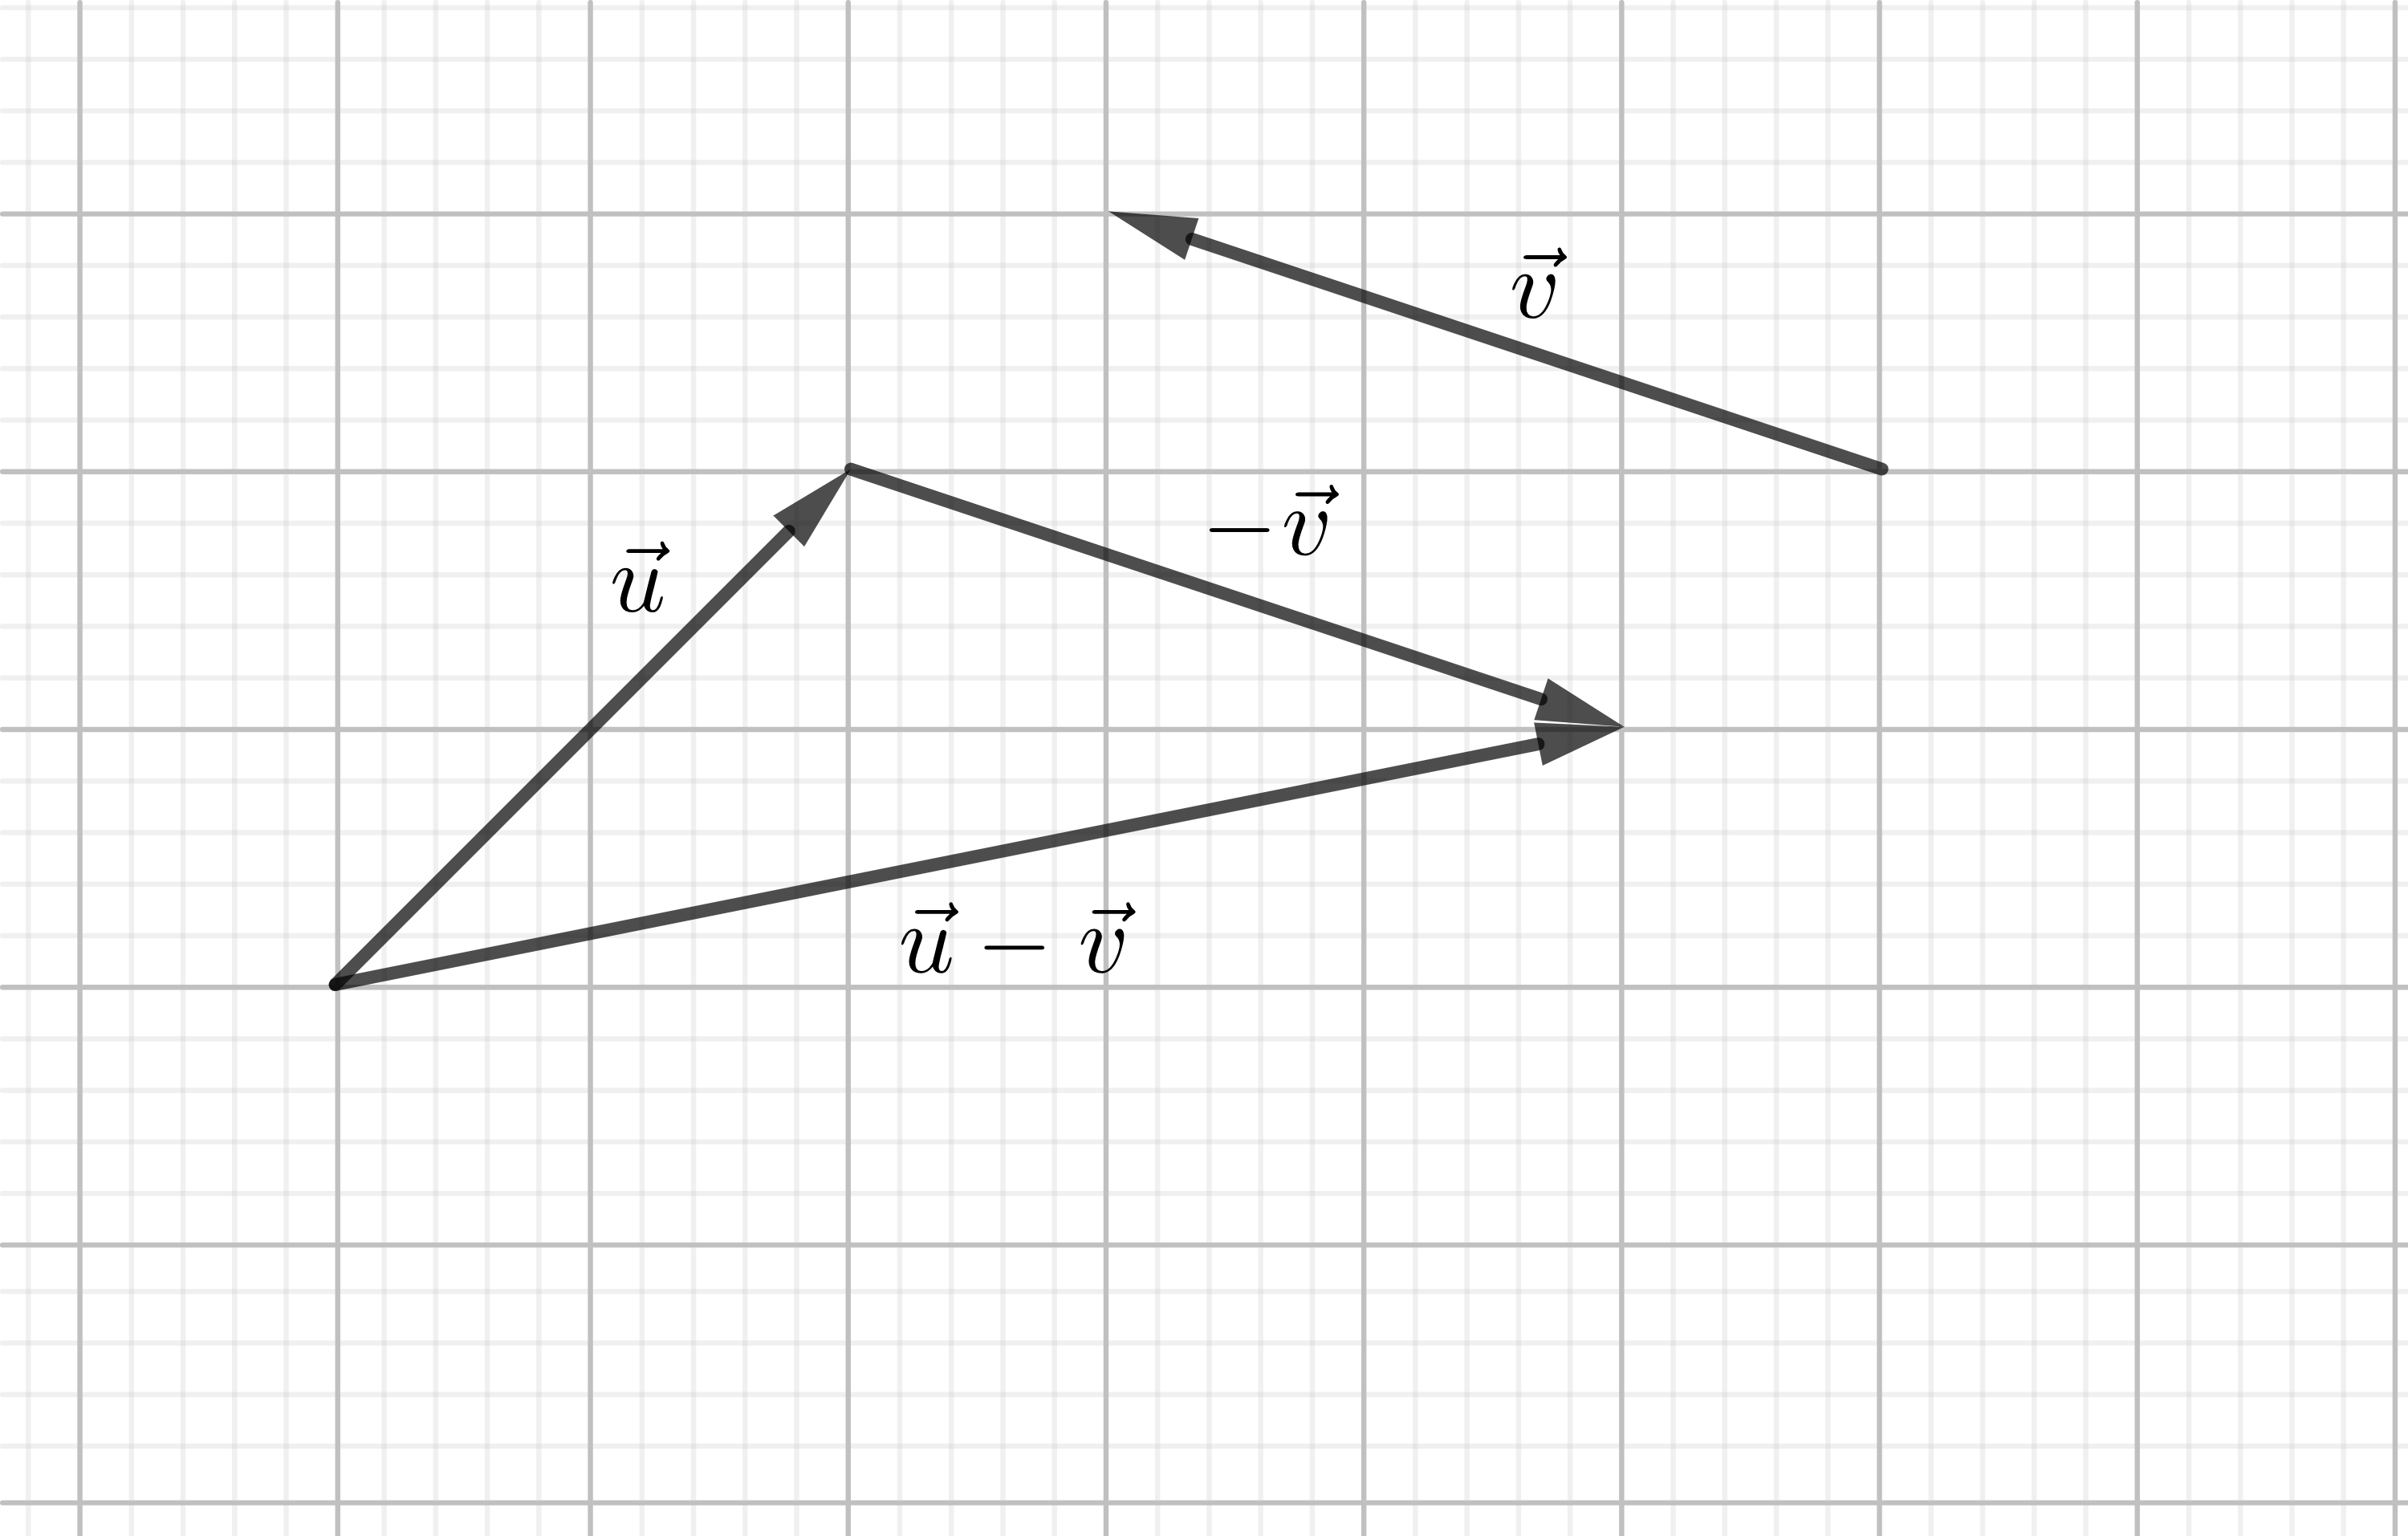
\includegraphics[width=0.5\textwidth]{./cap_vetor/dados/fig_vsubtracao/fig_vsubtracao}
  \caption{Representação geométrica da subtração de $\vec{u}$ com $\vec{v}$, i.e. $\vec{u}-\vec{v}$.}
  \label{fig:vsubtracao}
\end{figure}

\begin{obs}\normalfont{(Regra do paralelogramo)}\label{obs:vetor_regra_do_paralelogramo}
  \begin{flushright}
    \href{https://archive.org/details/regra-do-paralelogramo}{$\blacktriangleright$ Vídeo disponível!}
  \end{flushright}

  Sejam vetores não nulos $\vec{u} = \overrightarrow{AB}$ e $\vec{v} = \overrightarrow{AD}$. Seja, ainda, $C$ o vértice oposto ao $A$ no paralelogramo determinado pelos lados formados pelos segmentos $AB$ e $AD$. Então, temos $\vec{u} + \vec{v} = \overrightarrow{AC}$ e $\vec{u}-\vec{v} = \overrightarrow{DB}$. Veja a Figura \ref{fig:regrapara}.

\begin{figure}[H]
  \centering
  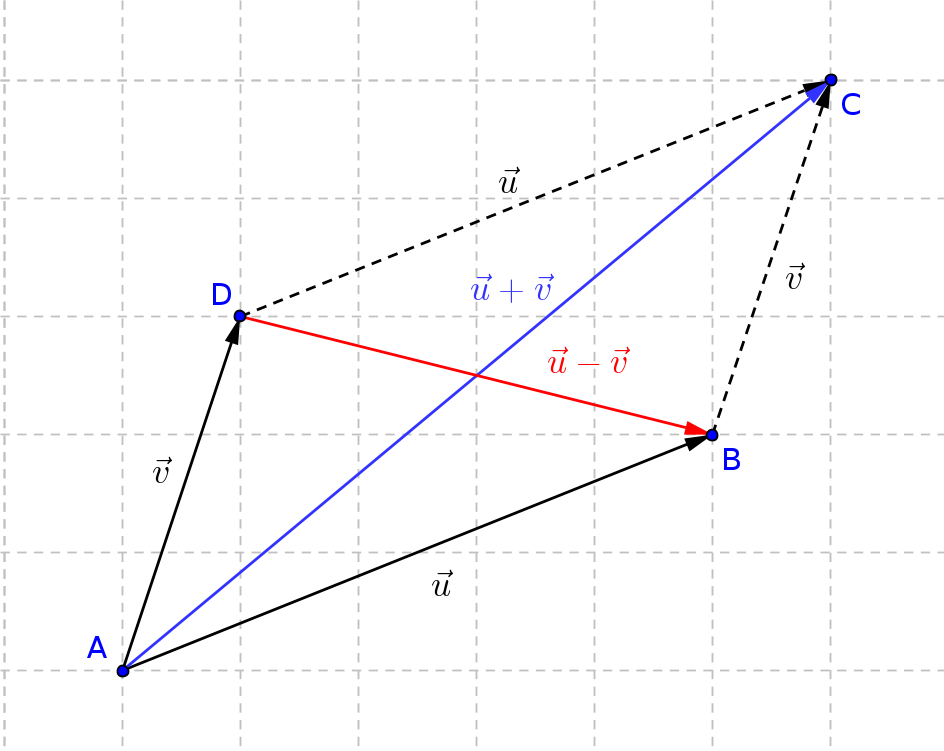
\includegraphics[width=0.6\textwidth]{./cap_vetor/dados/fig_regrapara/fig_regrapara}
  \caption{Regra do paralelogramo para a presentação geométrica da soma e da diferença de vetores.}
  \label{fig:regrapara}
\end{figure}  
\end{obs}

\subsection{Multiplicação de vetor por um escalar}

\begin{flushright}
  \href{https://archive.org/details/multiplicacao-vetor-por-escalar}{$\blacktriangleright$ Vídeo disponível!}
\end{flushright}

A multiplicação de um número real $\alpha>0$ (escalar) por um vetor $\vec{u}$ é denotado por $\alpha\vec{u}$ e é definido pelo vetor de mesma direção e mesmo sentido de $\vec{u}$ com norma $\alpha|\vec{u}|$. Quando $\alpha = 0$, define-se $\alpha\vec{u}=\vec{0}$, i.e. o vetor nulo (geometricamente, representado por qualquer ponto).

\begin{obs}
  Notamos que:
  \begin{itemize}
  \item Para $\alpha<0$, temos $\alpha\vec{u} = -(-\alpha\vec{u})$.
  \item $|\alpha\vec{u}|=|\alpha||\vec{u}|$.
\end{itemize}
\end{obs}

\begin{figure}[H]
  \centering
  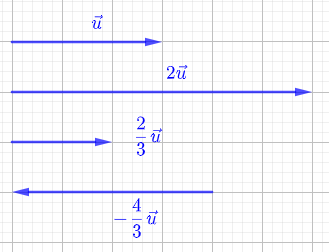
\includegraphics[width=0.6\textwidth]{./cap_vetor/dados/fig_vescalar/fig_vescalar}
  \caption{Representações geométricas de multiplicações de um vetor por diferentes escalares.}
  \label{fig:vescalar}
\end{figure}

\begin{obs}
  As seguintes propriedades são válidas:
  \begin{enumerate}[a)]
  \item Associatividade da multiplicação por escalar:
    \begin{equation}
      \alpha\left(\beta\vec{u}\right) = (\alpha\beta)\vec{u}
    \end{equation}

    De fato, em primeiro lugar, observamos que $\alpha\left(\beta\vec{u}\right)$ e $(\alpha\beta)\vec{u}$ têm a mesma direção e o mesmo sentido. Por fim, temos
    \begin{align}
      |\alpha\left(\beta\vec{u}\right)| &= |\alpha||\beta\vec{u}| \\
                                        &= |\alpha|\left(|\beta||\vec{u}|\right) \\
                                        &= \left(|\alpha||\beta|\right)|\vec{u}| \\
                                        &= |\alpha\beta||\vec{u}| \\
                                        &= |(\alpha\beta)\vec{u}|.
    \end{align}
    
  \item Distributividade:
    \begin{align}
      &(\alpha + \beta)\vec{u} = \alpha\vec{u} + \beta\vec{u}\\
      &\alpha\left(\vec{u}+\vec{v}\right) = \alpha\vec{u} + \alpha\vec{v}
    \end{align}
  \end{enumerate}
\end{obs}

\subsection{Resumo das propriedades das operações com vetores}

As operações de adição e multiplicação por escalar de vetores têm propriedades importantes. Para quaisquer vetores $\vec{u}$, $\vec{v}$ e $\vec{w}$ e quaisquer escalares $\alpha$ e $\beta$ temos:
\begin{itemize}
\item comutatividade da adição: $\vec{u}+\vec{v}=\vec{v}+\vec{u}$;
\item associatividade da adição: $(\vec{u} + \vec{v}) + \vec{w} = \vec{u} + (\vec{v} + \vec{w})$;
\item elemento neutro da adição: $\vec{u}+\vec{0}=\vec{u}$;
\item existência do oposto: $\vec{u}+(-\vec{u}) = \vec{0}$;
\item associatividade da multiplicação por escalar: $\alpha(\beta\vec{u})=(\alpha\beta)\vec{u}$;
\item distributividade da multiplicação por escalar:
  \begin{align}
    &\alpha(\vec{u}+\vec{v}) = \alpha\vec{u}+\alpha\vec{v},\\
    &(\alpha+\beta)\vec{u} = \alpha\vec{u}+\beta\vec{u};
  \end{align}
\item existência do elemento neutro da multiplicação por escalar: $1\vec{u}=\vec{u}$.
\end{itemize}

\subsection*{Exercícios resolvidos}

\begin{exeresol}
  Com base na figura abaixo, forneça o vetor $\overrightarrow{HC}$ como resultado de operações básicas envolvendo os vetores $\vec{u}$ e $\vec{v}$.
  \begin{figure}[H]
    \centering
    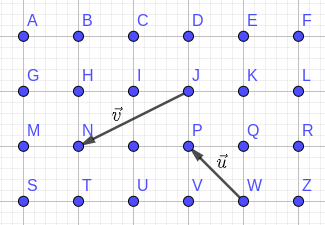
\includegraphics[width=0.7\textwidth]{./cap_vetor/dados/fig_exer_op_basicas/fig_vec_soma}
  \end{figure}
\end{exeresol}
\begin{resol}
  Vamos construir dois vetores auxiliares $\overrightarrow{HB}$ e $\overrightarrow{HI}$ a partir de operações envolvendo os vetores $\vec{u}$ e $\vec{v}$. Notamos que $\overrightarrow{HC} = \overrightarrow{HI} + \overrightarrow{HB}$.

  Começamos buscando formar o vetor $\overrightarrow{HI}$. Para tanto, observamos que $\vec{u}=\overrightarrow{NG}$ e, portanto, $\vec{v}+\vec{u}=\overrightarrow{JG}$. Com isso, obtemos que
  \begin{align}
    \overrightarrow{HI} &= -\frac{1}{3}\overrightarrow{JG} \\
                        &= -\frac{1}{3}(\vec{v}+\vec{u}).
  \end{align}

  Agora, vamos formar o vetor $\overrightarrow{HB}$. Isso pode ser feito da seguinte forma
  \begin{align}
    \overrightarrow{HB} &= \overrightarrow{WQ} \\
                        &= \vec{u} + \overrightarrow{PQ} \\
                        &= \vec{u} + \overrightarrow{HI} \\
                        &= \vec{u} -\frac{1}{3}(\vec{v}+\vec{u}) \\
                        &= \frac{2}{3}\vec{u} - \frac{1}{3}\vec{v}.
  \end{align}

  Por tudo isso, concluímos que
  \begin{align}
    \overrightarrow{HC} &= \overrightarrow{HI} + \overrightarrow{HB} \\
                        &= -\frac{1}{3}(\vec{v}+\vec{u}) \\
                        &+ \frac{2}{3}\vec{u} - \frac{1}{3}\vec{v} \\
                        &= \frac{1}{3}\vec{u} - \frac{2}{3}\vec{v}.
  \end{align}
\end{resol}

\begin{exeresol}\label{exeresol:vetor_comuta_adicao}
  Mostre que $\vec{u} + \vec{v} = \vec{v} + \vec{u}$.
\end{exeresol}
\begin{resol}
  Seja $ABCD$ o paralelogramo com $\vec{u} = \overrightarrow{AB} = \overrightarrow{DC}$ e $\vec{v} = \overrightarrow{AD} = \overrightarrow{BC}$. Logo, pela regra do paralelogramo temos
  \begin{align}
    \vec{u} + \vec{v} &= \overrightarrow{AB} + \overrightarrow{BC} \\
                      &= \overrightarrow{AC} \\
                      &= \overrightarrow{AD} + \overrightarrow{DC} \\
                      &= \vec{v} + \vec{u}.
  \end{align}
\end{resol}

\subsection*{Exercícios}

\begin{exer}
  Com base na figura abaixo, qual(is) dos vetores indicados são iguais ao vetor $\overrightarrow{AB}$.
  \begin{figure}[H]
    \centering
    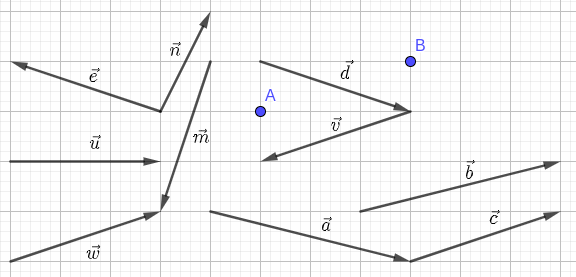
\includegraphics[width=0.7\textwidth]{./cap_vetor/dados/fig_exer_definicao_01/fig_exer_definicao_01}
  \end{figure}
\end{exer}
\begin{resp}
  $\vec{w}, \vec{c}$
\end{resp}

\begin{exer}
  Sejam $A$, $B$ e $C$ pontos dois a dois distintos. Se $\vec{b}$ é um vetor nulo, então $\vec{b}$ é igual a:
  \begin{enumerate}[a)]
  \item $\vec{0}$
  \item $\overrightarrow{AB}$
  \item $\overrightarrow{CC}$
  \item $\overrightarrow{CA}$
  \item $\overrightarrow{BB}$
  \end{enumerate}
\end{exer}
\begin{resp}
  a), c), e) 
\end{resp}

\begin{exer}
  Com base na figura abaixo, qual(is) dos vetores indicados são paralelos entre si.
  \begin{figure}[H]
    \centering
    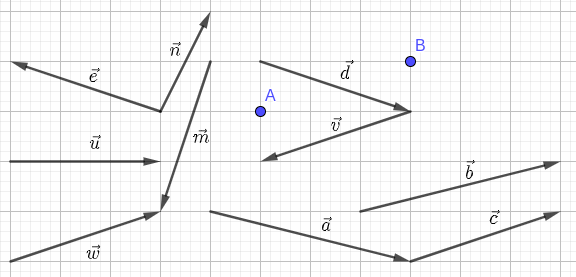
\includegraphics[width=0.7\textwidth]{./cap_vetor/dados/fig_exer_definicao_01/fig_exer_definicao_01}
  \end{figure}
\end{exer}
\begin{resp}
  $\vec{d}\parallel\vec{e}$; $\vec{c}\parallel\vec{v}\parallel\vec{w}$
\end{resp}

\begin{exer}
  Com base na figura abaixo, qual(is) dos vetores indicados são ortogonais (perpendiculares) entre si.
  \begin{figure}[H]
    \centering
    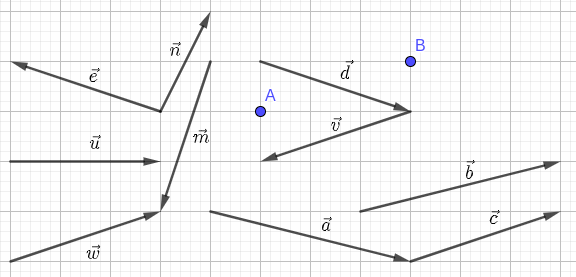
\includegraphics[width=0.7\textwidth]{./cap_vetor/dados/fig_exer_definicao_01/fig_exer_definicao_01}
  \end{figure}
\end{exer}
\begin{resp}
  $\vec{e}\perp\vec{n}$; $\vec{d}\perp\vec{n}$; $\vec{a}\perp\vec{m}$
\end{resp}

\begin{exer}
  Com base na figura abaixo, qual(is) dos seguintes são representações do vetor $\overrightarrow{v}+\overrightarrow{u}$?
  \begin{enumerate}[a)]
  \item $\overrightarrow{JG}$
  \item $\overrightarrow{QN}$
  \item $\overrightarrow{AD}$
  \item $\overrightarrow{JV}$
  \item $\overrightarrow{NN}$
  \end{enumerate}
  \begin{figure}[H]
    \centering
    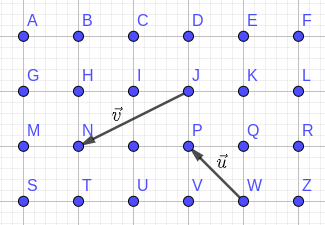
\includegraphics[width=0.7\textwidth]{./cap_vetor/dados/fig_exer_op_basicas/fig_vec_soma}
  \end{figure}
\end{exer}
\begin{resp}
  a), b)
\end{resp}

\begin{exer}
  Com base na figura abaixo, qual(is) dos seguintes são representações do vetor $\vec{w}+\vec{v}+\vec{u}$?
  \begin{enumerate}[a)]
  \item $\overrightarrow{0}$
  \item $\overrightarrow{SP}$
  \item $\overrightarrow{FP}$
  \item $\overrightarrow{v}$
  \item $\overrightarrow{AD}$
  \end{enumerate}
  \begin{figure}[H]
    \centering
    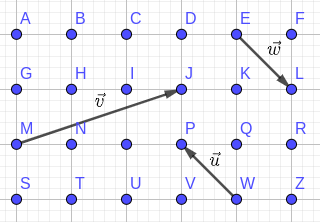
\includegraphics[width=0.7\textwidth]{./cap_vetor/dados/fig_exer_op_basicas/fig_vec_assop}
  \end{figure}
\end{exer}
\begin{resp}
  b), d)
\end{resp}

\begin{exer}
  Com base na figura abaixo, escreva os seguintes vetores como resultado de operações envolvendo $\vec{u}$ ou $\vec{v}$.
  \begin{enumerate}[a)]
  \item $\overrightarrow{QK}$
  \item $\overrightarrow{KI}$
  \item $\overrightarrow{TO}$
  \item $\overrightarrow{PE}$
  \item $\overrightarrow{FT}$
  \end{enumerate}
  \begin{figure}[H]
    \centering
    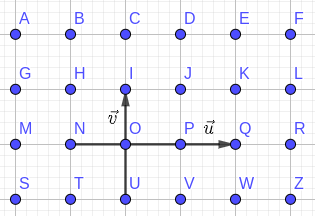
\includegraphics[width=0.7\textwidth]{./cap_vetor/dados/fig_exer_op_basicas/fig_vec_comb}
  \end{figure}
\end{exer}
\begin{resp}
  a)~$\frac{1}{2}\vec{v}$; b)~$-\frac{2}{3}\vec{u}$; c)~$\frac{1}{2}\vec{v}+\frac{1}{3}\vec{u}$; d)~$\vec{v}+\frac{1}{3}\vec{u}$; e)~$-\frac{4}{3}\vec{u}-\frac{3}{2}\vec{v}$
\end{resp}


\begin{exer}
  Seja dado um vetor $\vec{u}\neq 0$. Calcule a norma do vetor $\vec{v}=\vec{u}/|\vec{u}|$\footnote{$\vec{u}/|\vec{u}|$ é chamado de vetor $\vec{u}$ normalizado, ou a normalização do vetor $\vec{u}$.}.
\end{exer}
\begin{resp}
  $|\vec{v}|=1$.
\end{resp}

\begin{exer}
  Diga se é verdadeira ou falsa cada uma das seguintes afirmações. Justifique sua resposta.
  \begin{enumerate}
  \item $\vec{u}+\vec{u} = 2\vec{u}$
  \item $\vec{u}=-\vec{u} \Leftrightarrow \vec{u} = \vec{0}$.
  \end{enumerate}
\end{exer}
\begin{resp}
  a) verdadeira; b) verdadeira.
\end{resp}
